\section{Introduction}
\label{sec:Intro}

\subsection{Background Information}
\label{subsec:BackgroundInfo}

This document describes the architecture, design, and implementation for the popular game MineSweeper.
\href{https://en.wikipedia.org/wiki/Minesweeper_(video_game)}{See Here} for more information.
The project was done in Unity and utilized the usage of several scripts as well as assets which are acknowledged within the Acknowledgements section at the end of this document.

The title for this project: \textbf{MineSweeper 3D} is named so due to the project utilizing 3D elements to construct the game.
Each cell within the visible board is a 3D element which casts shadows and reflects light.
Not all elements, however, within the game utilize 3D structures, e.g., the menus.

This project offers players a new take on the classic game of MineSweeper by expanding into the \nth{3} dimension.

\subsection{Project Information}
\label{subsec:ProjInfo}

This project addresses the interests of the major stakeholders including:
\begin{itemize}
    \item The professor --- wants a project that utilizes modern software development techniques, game design strategies, and smart application of the ideas discussed in class.
    Additonally, there is the desire for quality code design, precise implementation, and unambiguous documentation leading into the fulfillment of Software Development Tasks such as usability, reliability, etc.
    \item Players of the game --- they want a functioning product with thoughtful insight into the design and playability of the game. The game should be as bug-free as possible. Furthermore, the game should be fun.
    \item The Developer --- wants the code to be properly structured, commented, and legible. 
    On top of maintaining high quality code, the elements within the various parts of the project not in code (those within the Unity Design Window) should also be held to the same caliber.
\end{itemize}

The design of this project is highly complicated and necessitates the documentation to descrbe the project from a variety of perspectives:
\begin{enumerate}
    \item Logical View --- components accompanied by their operations and attributes. Additionally, the relationships between the components amongst other components.
    \item Process View --- the processes that handle execution for components described in the Logical View
    \item Development View --- the larger scale view of the project including those described in the Process and Logical Views.
    \item Use Case View --- describe the end user interactions with the system. 
    These serve as both a guideline for project construction as well as defining the user requirements.
\end{enumerate}

\subsection{Game Information}
\label{subsec:GameInfo}

The Rules to play this game can be seen below in Figure \ref{Fig:HowToPlay}. These are locationed on the publicly visible Github Repository seen \href{https://github.com/EZRA-DVLPR/MineSweeper3D}{here}.
Also located on the Github Repository is a ReadMe file which describes the process for downloading and playing the game for oneself.

\begin{figure}[h]
    \centering
    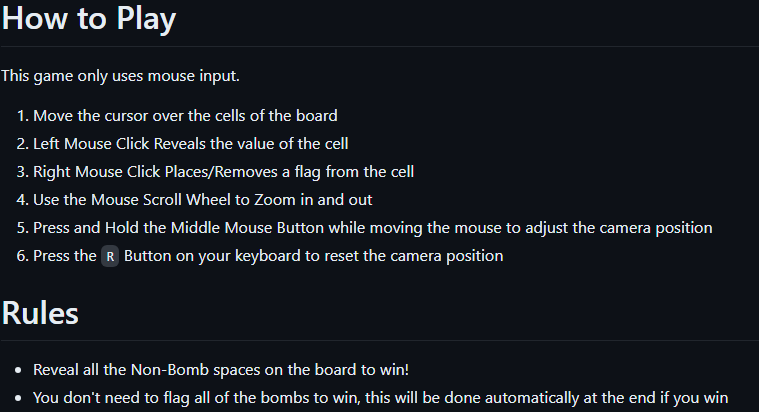
\includegraphics[width=10cm]{Images/HowToPlay.png}
       \caption{The rules of the game and how to play.}
           \label{Fig:HowToPlay}
\end{figure}